\chapter{Étude expérimentale}

\section{Complexité théorique de l'algorithme de résolution}
\paragraph{Complexité temporelle}
La complexité de l'algorithme de résolution comme calculée précédemment est de l'ordre de $\mathcal{O}(2^{n})$, et elle est précisément égale à $2^{n} - 1$ qui est une complexité exponentielle.
\par
Le tableau suivant représente les temps d'exécution théorique en nanoseconde de l'algorithme de résolution selon la variation de la taille du problème (le nombre de disques) :

\small
\begin{center}
    \resizebox{\textwidth}{!}{
        \begin{tabular}{| c | c | c | c | c | c | c | c | c | c | c | c | c |}
            \hline
            N & 1 & 10 & 50 & 100 & 150 & 250 & 500 & 750 & 1000\\
            \hline
            t(ns) & 2 & 1024 & 1,1259E+15 & 1,26765E+30 & 1,42725E+4 & 1,80925E+75 & 3,27339E+150 & 5,92239E+225 & 1,07151E+301\\
            \hline
        \end{tabular}
    }
\end{center}

La figure suivante (voir Figure \ref{fig:temps_exec_th_algo_reso}) représente l'évolution du temps d'exécution théorique selon le nombre de disques :

\begin{figure}[H]
    \centering
        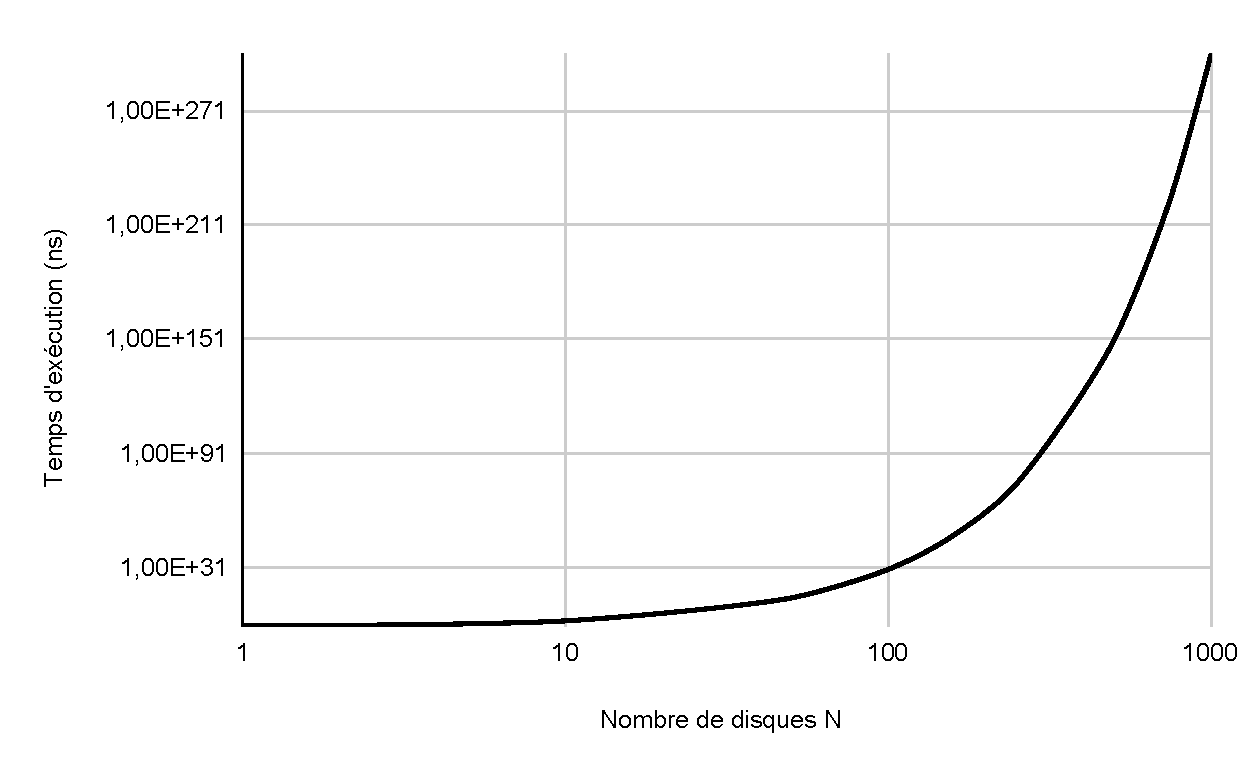
\includegraphics[scale=0.5]{./ressources/temps_execution_th_algo_reso.pdf}
        \caption{Temps d'exécution théorique de l'algorithme de résolution}
    \label{fig:temps_exec_th_algo_reso}
\end{figure} 

Depuis le graphe, on observe que le temps d'exécution évolue de manière exponentielle selon le nombre de disques de départ. Il atteint rapidement des temps d'exécution incommensurables le rendant inexploitable.

\paragraph{Complexité spatiale}
L'algorithme exploite une matrice $3 x n$ tel que $n$ est le nombre de disques. Chaque disque est représenté par un entier de taille $4$ octets. De plus, la taille de la représentation est stattique au cours de l'exécution. Par conséquent, la complexité spatiale est égale à $4 * 3 * n$ octets donc de l'ordre de $\mathcal{O}(n)$.
\par
Cependant, l'algorithme récursif fait au maximum $n$ appels récursifs (le nombre maximum d'appels est le nombre maximum de disques pouvant être déplacés à la fois). L'adresse de retour étant stockée sur $8$ octets, la taille maximal de la pile d'appel de fonctions exploitée est donc égale à $8 * n$ octets qui est de l'ordre de $\mathcal{O}(n)$.
\par
La complexité spatiale totale est donc de l'ordre de $\mathcal{O}(n)$.

\section{Complexité théorique de l'algorithme de vérification}
\paragraph{Complexité temporelle}
La complexité temporelle de l'algorithme de vérification est linéaire et elle est égale à $n \cong \mathcal{O}(n)$.
\paragraph{Complexité spatiale}
La complexité spatiale de l'algorithme de vérification est égale à la taille de la matrice, c.à.d. $3 * n$ donc de l'ordre $\mathcal{O}(n)$.
